\documentclass[margin=5mm]{standalone}
\usepackage[dvipsnames]{xcolor}
\usepackage{pgfplots}
\usepackage{tikz}
\usepackage[tikz]{ocgx2}

\pgfplotsset{compat=1.18}
\begin{document}

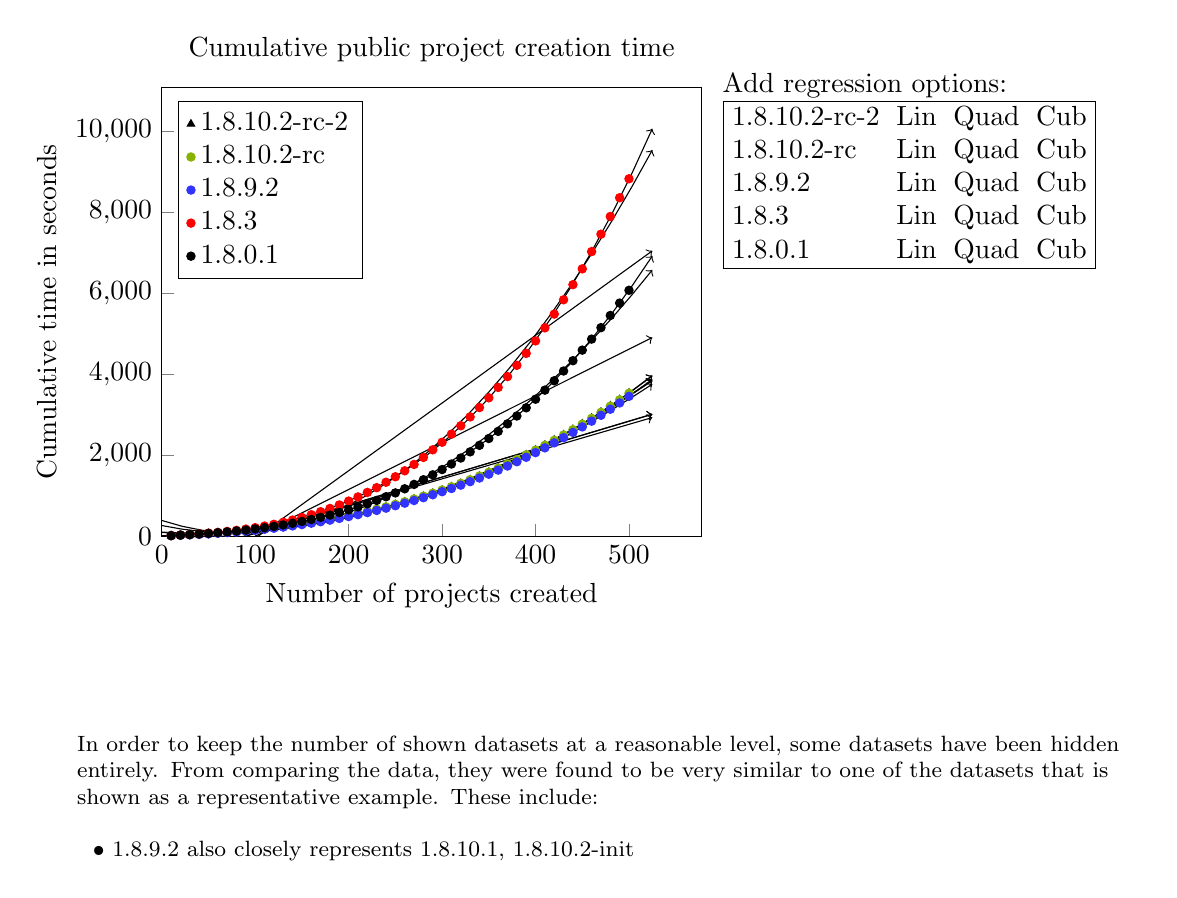
\begin{tikzpicture}
    \begin{axis}[
        align = center,
        legend pos = north west,
        legend cell align = left,
        xlabel = Number of projects created,
        ylabel = Cumulative time in seconds,
        xtick pos = left,
        ytick pos = left,
        scaled ticks = false,
        xmin = 0,
        ymin = 0,
        title = {Cumulative public project creation time},
        title style = {text width = 0.8\textwidth},
        legend entries={\switchocg{1.8.10.2-rc-2}{1.8.10.2-rc-2},\switchocg{1.8.10.2-rc}{1.8.10.2-rc},\switchocg{1.8.9.2}{1.8.9.2},\switchocg{1.8.3}{1.8.3},\switchocg{1.8.0.1}{1.8.0.1}}]
        \begin{scope}[ocg = {ref = 1.8.10.2-rc-2-Lin, status = invisible}]
            \plot[domain=0:525,->,forget plot] (\x,{-616.17039755102086928673088550567626953125 + 6.92454493157263062386164165218360722064971923828125*(\x)^1});
        \end{scope}
        \begin{scope}[ocg = {ref = 1.8.10.2-rc-2-Quad, status = invisible}]
            \plot[domain=0:525,->,forget plot] (\x,{93.0154090816328249502475955523550510406494140625 + -1.2583682218810581243673141216277144849300384521484375*(\x)^1 + 0.0160449277518699730260554048300036811269819736480712890625*(\x)^2});
        \end{scope}
        \begin{scope}[ocg = {ref = 1.8.10.2-rc-2-Cub, status = invisible}]
            \plot[domain=0:525,->,forget plot] (\x,{5.98523049500592119187558637349866330623626708984375 + 0.6934269981078682310027261337381787598133087158203125*(\x)^1 + 0.00657139597538671134391297101728923735208809375762939453125*(\x)^2 + 0.00001238370166860556611837691776134562360311974771320819854736328125*(\x)^3});
        \end{scope}
        \begin{scope}[ocg = {ref = 1.8.10.2-rc-2, status = visible}]
            \addplot[
                only marks,
                color = black,
                mark = triangle*,
                mark size = 1.5 pt
            ]coordinates {(10,11.58)(20,21.565)(30,32.288)(40,45.05)(50,59.669)(60,74.751)(70,91.548)(80,109.975)(90,131.03)(100,153.019)(110,177.307)(120,208.362)(130,237.178)(140,267.7)(150,301.144)(160,335.827)(170,373.788)(180,415.074)(190,459.505)(200,505.629)(210,554.934)(220,607.476)(230,663.852)(240,722.078)(250,783.369)(260,848.272)(270,916.021)(280,986.638)(290,1060.964)(300,1138.375)(310,1220.316)(320,1305.196)(330,1394.353)(340,1486.508)(350,1582.884)(360,1683.821)(370,1788.072)(380,1896.702)(390,2013.3)(400,2131.015)(410,2251.737)(420,2376.637)(430,2505.933)(440,2639.886)(450,2778.901)(460,2920.97)(470,3069.002)(480,3221.424)(490,3378.644)(500,3540.159)};
        \end{scope}
        \begin{scope}[ocg = {ref = 1.8.10.2-rc-Lin, status = invisible}]
            \plot[domain=0:525,->,forget plot] (\x,{-606.4355706122447600137093104422092437744140625 + 6.895337767106841653230731026269495487213134765625*(\x)^1});
        \end{scope}
        \begin{scope}[ocg = {ref = 1.8.10.2-rc-Quad, status = invisible}]
            \plot[domain=0:525,->,forget plot] (\x,{96.762391122449827207674388773739337921142578125 + -1.21848486829347191218175794347189366817474365234375*(\x)^1 + 0.015909456147843746565140321536091505549848079681396484375*(\x)^2});
        \end{scope}
        \begin{scope}[ocg = {ref = 1.8.10.2-rc-Cub, status = invisible}]
            \plot[domain=0:525,->,forget plot] (\x,{5.33297691272248730598448673845268785953521728515625 + 0.8319704624778931911777135610464029014110565185546875*(\x)^1 + 0.005957052569136229470958543430469944723881781101226806640625*(\x)^2 + 0.000013009677880663415207459186750948987310039228759706020355224609375*(\x)^3});
        \end{scope}
        \begin{scope}[ocg = {ref = 1.8.10.2-rc, status = visible}]
            \addplot[
                only marks,
                color = lime!70!black,
                mark = *,
                mark size = 1.5 pt
            ]coordinates {(10,12.689)(20,24.025)(30,36.894)(40,49.989)(50,63.609)(60,78.501)(70,96.29)(80,114.844)(90,135.442)(100,162.486)(110,187.455)(120,215.16)(130,244.976)(140,276.747)(150,310.038)(160,345.553)(170,383.77)(180,424.869)(190,468.625)(200,513.841)(210,562.003)(220,613.551)(230,668.54)(240,726.806)(250,787.844)(260,851.605)(270,919.357)(280,989.924)(290,1063.688)(300,1140.74)(310,1222.09)(320,1307.395)(330,1395.979)(340,1487.897)(350,1583.185)(360,1683.608)(370,1787.119)(380,1895.144)(390,2010.488)(400,2126.446)(410,2247.262)(420,2371.318)(430,2500.648)(440,2634.416)(450,2772.138)(460,2914.818)(470,3061.736)(480,3214.581)(490,3372.401)(500,3535.248)};
        \end{scope}
        \begin{scope}[ocg = {ref = 1.8.9.2-Lin, status = invisible}]
            \plot[domain=0:525,->,forget plot] (\x,{-604.357680816326364947599358856678009033203125 + 6.7404327875150062965303732198663055896759033203125*(\x)^1});
        \end{scope}
        \begin{scope}[ocg = {ref = 1.8.9.2-Quad, status = invisible}]
            \plot[domain=0:525,->,forget plot] (\x,{96.1630798979606566945221857167780399322509765625 + -1.34249906688060338666446114075370132923126220703125*(\x)^1 + 0.0158488859890109946848557598286788561381399631500244140625*(\x)^2});
        \end{scope}
        \begin{scope}[ocg = {ref = 1.8.9.2-Cub, status = invisible}]
            \plot[domain=0:525,->,forget plot] (\x,{7.2395928310908370661991284578107297420501708984375 + 0.6517567168083544526524519824306480586528778076171875*(\x)^1 + 0.006169261126869944773798426496114188921637833118438720703125*(\x)^2 + 0.000012653104394955613765626212252612958764075301587581634521484375*(\x)^3});
        \end{scope}
        \begin{scope}[ocg = {ref = 1.8.9.2, status = visible}]
            \addplot[
                only marks,
                color = blue!80!white,
                mark = *,
                mark size = 1.5 pt
            ]coordinates {(10,12.503)(20,21.753)(30,31.869)(40,43.994)(50,57.519)(60,72.379)(70,89.069)(80,106.649)(90,125.998)(100,147.499)(110,170.796)(120,196.69)(130,224.481)(140,254.7)(150,286.864)(160,321.142)(170,357.685)(180,397.061)(190,439.632)(200,484.285)(210,533.148)(220,583.571)(230,636.819)(240,693.341)(250,753.033)(260,815.892)(270,881.775)(280,951.732)(290,1024.043)(300,1099.779)(310,1178.815)(320,1261.358)(330,1348.011)(340,1438.05)(350,1532.182)(360,1633.739)(370,1735.039)(380,1840.899)(390,1951.247)(400,2065.758)(410,2184.085)(420,2308.33)(430,2434.866)(440,2566.459)(450,2702.259)(460,2844.322)(470,2989.356)(480,3139.242)(490,3294.605)(500,3458.311)};
        \end{scope}
        \begin{scope}[ocg = {ref = 1.8.3-Lin, status = invisible}]
            \plot[domain=0:525,->,forget plot] (\x,{-1726.456342857141862623393535614013671875 + 16.729666756302517427457132725976407527923583984375*(\x)^1});
        \end{scope}
        \begin{scope}[ocg = {ref = 1.8.3-Quad, status = invisible}]
            \plot[domain=0:525,->,forget plot] (\x,{389.6393826530666046892292797565460205078125 + -7.6868223841998588596879926626570522785186767578125*(\x)^1 + 0.04787546890294581969360621087616891600191593170166015625*(\x)^2});
        \end{scope}
        \begin{scope}[ocg = {ref = 1.8.3-Cub, status = invisible}]
            \plot[domain=0:525,->,forget plot] (\x,{2.031504598353338852945171311148442327976226806640625 + 1.0059232346571060912054917935165576636791229248046875*(\x)^1 + 0.0056830293469178373710892770986902178265154361724853515625*(\x)^2 + 0.0000551535157595136821067315080480142341912142001092433929443359375*(\x)^3});
        \end{scope}
        \begin{scope}[ocg = {ref = 1.8.3, status = visible}]
            \addplot[
                only marks,
                color = red,
                mark = *,
                mark size = 1.5 pt
            ]coordinates {(10,17.008)(20,28.977)(30,42.754)(40,58.713)(50,75.606)(60,95.22)(70,118.639)(80,144.939)(90,175.71)(100,210.514)(110,250.693)(120,294.509)(130,344.707)(140,399.709)(150,462.373)(160,531.451)(170,605.418)(180,686.141)(190,772.827)(200,868.767)(210,970.67)(220,1082.181)(230,1200.262)(240,1334.171)(250,1470.011)(260,1617.298)(270,1774.106)(280,1948.092)(290,2136.407)(300,2322.439)(310,2523.407)(320,2731.308)(330,2950.221)(340,3179.977)(350,3421.752)(360,3678.466)(370,3945.736)(380,4225.127)(390,4520.607)(400,4828.741)(410,5151.528)(420,5492.104)(430,5845.659)(440,6219.769)(450,6610.35)(460,7036.968)(470,7467.596)(480,7904.933)(490,8368.659)(500,8837.214)};
        \end{scope}
        \begin{scope}[ocg = {ref = 1.8.0.1-Lin, status = invisible}]
            \plot[domain=0:525,->,forget plot] (\x,{-1155.934110204081889605731703341007232666015625 + 11.557391020408164905575176817364990711212158203125*(\x)^1});
        \end{scope}
        \begin{scope}[ocg = {ref = 1.8.0.1-Quad, status = invisible}]
            \plot[domain=0:525,->,forget plot] (\x,{263.62972295918569898276473395526409149169921875 + -4.8221916699372133763290548813529312610626220703125*(\x)^1 + 0.032116828804598769597777874196253833360970020294189453125*(\x)^2});
        \end{scope}
        \begin{scope}[ocg = {ref = 1.8.0.1-Cub, status = invisible}]
            \plot[domain=0:525,->,forget plot] (\x,{9.657371059487243059038519277237355709075927734375 + 0.87355698297140371710867157162283547222614288330078125*(\x)^1 + 0.004471072066605716148479654492575718904845416545867919921875*(\x)^2 + 0.0000361382441019516835087853345864772336426540277898311614990234375*(\x)^3});
        \end{scope}
        \begin{scope}[ocg = {ref = 1.8.0.1, status = visible}]
            \addplot[
                only marks,
                color = black,
                mark = *,
                mark size = 1.5 pt
            ]coordinates {(10,14.625)(20,28.368)(30,41.079)(40,55.327)(50,70.008)(60,86.47)(70,105.983)(80,127.594)(90,151.039)(100,178.977)(110,208.377)(120,242.625)(130,279.09)(140,320.098)(150,364.669)(160,413.641)(170,466.002)(180,522.594)(190,584.63)(200,651.092)(210,723.725)(220,801.212)(230,883.982)(240,975.248)(250,1070.342)(260,1172.324)(270,1280.676)(280,1396.001)(290,1517.89)(300,1647.91)(310,1784.951)(320,1933.025)(330,2085.372)(340,2246.555)(350,2415.053)(360,2592.313)(370,2778.318)(380,2971.754)(390,3174.547)(400,3386.797)(410,3611.099)(420,3843.169)(430,4084.435)(440,4339.708)(450,4600.634)(460,4873.212)(470,5156.588)(480,5456.902)(490,5763.631)(500,6080.369)};
        \end{scope}
    \end{axis}
    \begin{scope}
        \addtolength{\tabcolsep}{-0.3em}
        \node [below right, shape=rectangle, align=left](regressiontable) at (7,6) {
            Add regression options: \\
            \begin{tabular}{|llll|}
                \hline
                1.8.10.2-rc-2 & \switchocg{1.8.10.2-rc-2-Lin}{Lin} & \switchocg{1.8.10.2-rc-2-Quad}{Quad} & \switchocg{1.8.10.2-rc-2-Cub}{Cub} \\
                1.8.10.2-rc & \switchocg{1.8.10.2-rc-Lin}{Lin} & \switchocg{1.8.10.2-rc-Quad}{Quad} & \switchocg{1.8.10.2-rc-Cub}{Cub} \\
                1.8.9.2 & \switchocg{1.8.9.2-Lin}{Lin} & \switchocg{1.8.9.2-Quad}{Quad} & \switchocg{1.8.9.2-Cub}{Cub} \\
                1.8.3 & \switchocg{1.8.3-Lin}{Lin} & \switchocg{1.8.3-Quad}{Quad} & \switchocg{1.8.3-Cub}{Cub} \\
                1.8.0.1 & \switchocg{1.8.0.1-Lin}{Lin} & \switchocg{1.8.0.1-Quad}{Quad} & \switchocg{1.8.0.1-Cub}{Cub} \\
                \hline
            \end{tabular}
        };
    \end{scope}
    \begin{scope}[every node/.style = {font=\footnotesize}, right]
        \node[text width = 13.5 cm] at (-1.2,-3) {In order to keep the number of shown datasets at a reasonable level, some datasets have been hidden entirely. From comparing the data, they were found to be very similar to one of the datasets that is shown as a representative example. These include:};
        \node at (-1,-4.0) {$\bullet$ 1.8.9.2 also closely represents 1.8.10.1, 1.8.10.2-init};
    \end{scope}
\end{tikzpicture}

\end{document}